\subsection{Apache Airflow™}

Apache Airflow™ stands as an open-source platform designed to manage data flow within systems associated with data. In the face of the escalating challenge of data pipeline management, Airflow emerges as a comprehensive solution, automating and optimizing data-related workflows effectively \cite{airflow}.

Airflow not only aids in defining and managing the start and end times of each data pipeline but also provides precise and detailed monitoring of the results of each task. This becomes particularly crucial when ensuring the integrity and reliability of the processed data.

With the ability to discern complex relationships between tasks through the Directed Acyclic Graph (DAG) model, Airflow empowers administrators with tighter control and flexibility in handling workflow processes. Its robust integration with logging systems facilitates detailed activity tracking, assisting in issue resolution and ensuring that every process aligns with expectations.

Simultaneously, the scheduling flexibility makes Airflow an excellent tool for time and resource management. Its strong integration with various data sources and extensibility through plugins allows Airflow to meet diverse needs in data processing and task automation.

Apache Airflow not only delivers robust performance but also brings flexibility and optimal technical features to data processing workflows. With its time management capabilities, powerful logging integration, scheduling flexibility, and scalability, Airflow stands as the top choice for enhancing performance and control in data processing workflows.

\subsection{Kubernetes}

Kubernetes, an open-source system for managing and deploying highly flexible applications in cloud and data center environments,
has evolved into one of the most widely adopted tools in the field of Information Technology \cite{k8s-doc}.
Originally developed by Google and later transferred to the Cloud Native Computing Foundation (CNCF),
Kubernetes aims to automate the deployment, scaling, and management of containerized applications, alleviating the burden on developers and system administrators. The platform offers a unified foundation for deploying, scaling, and managing containerized applications across multiple servers.

Kubernetes operates based on key concepts such as Pods, Services, ReplicaSets, and various other abstractions, creating a flexible environment for application deployment and management. This fosters an environment where developers can easily build applications, and system administrators can efficiently maintain them.

Beyond supporting traditional deployment models, Kubernetes paves the way for innovative strategies like Continuous Deployment (CD) and Microservices. With the ability to automate many aspects of the development and deployment process, Kubernetes plays a crucial role in constructing and sustaining complex, flexible, and scalable systems.

\subsubsection{Kubernetes Components}

Introducing essential concepts for managing and deploying applications, Kubernetes provides an effective and flexible environment. The main components of Kubernetes include Pod, ReplicaSet, Deployment, and Service.

\begin{figure}[H]
    \centering
    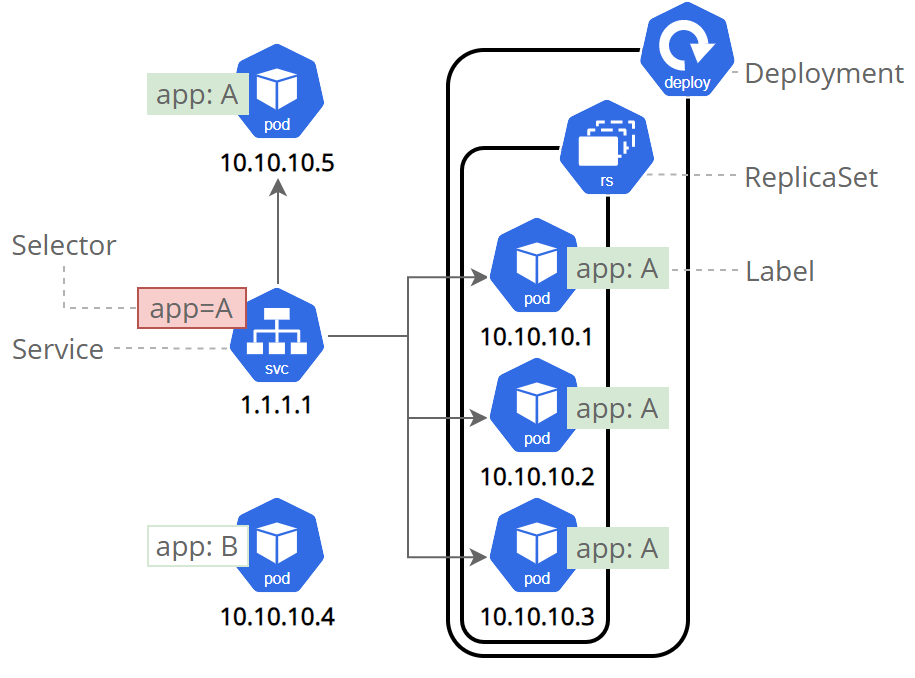
\includegraphics[width=0.75\linewidth]{Images/3.4-k8s-comps.png}
    \caption{Overview of Kubernetes Components - Kubernetes}
    \label{fig:k8s-comps}
\end{figure}

In Kubernetes, a \textbf{Pod} serves as the fundamental unit, representing a collection of containers that share a common workspace.
Within the same Pod, containers collaborate by sharing network and storage resources, fostering interaction and enabling the construction of intricate applications.

The \textbf{ReplicaSet}, a crucial resource in Kubernetes, ensures a designated number of Pods operate in a specified manner.
In the event of a Pod failure or shutdown, the ReplicaSet automatically initiates the creation of a new Pod to replace it.
This mechanism ensures the application's stable state by guaranteeing a defined number of Pods are consistently operational.

For managing the deployment and updating processes of applications, \textbf{Deployment} is a key component in Kubernetes.
It articulates the desired state of the application and orchestrates the updating of the ReplicaSet to achieve that state.
Deployment provides versatile management capabilities, facilitating the deployment of new versions, rollbacks, and updates without disrupting the service.

The \textbf{Service} resource in Kubernetes furnishes an HTTP port to Pods, generating a unique IP address and DNS name for a cluster of Pods.
This enables seamless communication among applications within the cluster and with external environments.
Service effectively simplifies the intricacies of handling multiple Pods and IP addresses, offering a straightforward means of accessing services within the Kubernetes environment.

Typically, large-scale systems leverage Kubernetes in their software development and deployment processes.
This adoption brings several advantages, including efficient resource management and self-recovery capabilities.
Kubernetes optimizes resource utilization, ensuring optimal performance and reducing waste.
Additionally, it automatically addresses issues during operations, enhancing high availability.

However, the technology is not without its challenges, including a steep learning curve for beginners.
Mastery of diverse knowledge areas such as computer networking and containerization is necessary.
Moreover, deploying and maintaining Kubernetes demands significant resources, both in terms of personnel and hardware, particularly for smaller organizations.

\subsubsection{High Availability in Kubernetes}

High Availability is a crucial factor in the success of any system. In Kubernetes, High Availability is achieved through the combination of several features, including self-healing, load balancing, and auto-scaling.

First, Kubernetes uses \textbf{Deployment}, a type of \textbf{Controller} for managing replicas.
Through Deployment, we can easily perform horizontal scaling, which is the process of increasing the number of replicas of a Pod.
This mechanism ensures that the application can handle numerous requests without compromising performance.
Moreover, in case of a Pod failure, a Deployment makes sure that a new Pod is created to replace it, ensuring the amounts of predefined replicas is always maintained.

At network layers, Kubernetes uses \textbf{Service} for communication between various components within or outside the cluster.
Instead of directly accessing Pods, other components can access Services, which will redirect the request to the appropriate Pod.
When Pods are replaced, the Service will automatically update the routing rules to ensure the request is sent to the correct Pod.
Outside the cluster, Kubernetes also uses \textbf{Ingress} to manage external access to Services.
Instead of specifying the direct node IP address, Clients can abstract it by using only the URL or hostname.

Finally, at the storage level, Kubernetes provides Persistent Volumes.
By doing so, applications can be agnostic to the underlying storage infrastructure.
This allows for easier management and scaling of storage resources.
Not only that, depending on the provided \textbf{Storage Class}, Kubernetes makes sure that the data is replicated to multiple nodes,
ensuring data availability in case of node failure.

To summarize, Kubernetes provides a robust set of features to ensure High Availability.
By leveraging these features, we can build a highly available system that can scale with our load, while also being resilient to failures.

\subsection{LROSE}

LROSE (Lidar Radar Open Software Environment) is a project supported by the National Science Foundation (NSF) with the goal of developing common software for the Lidar, Radar, and Profiler community. The project operates based on the principles of collaboration and open source. The core software package of LROSE is a collaborative effort between Colorado State University (CSU) and the Earth Observing Laboratory (EOL) at the National Center for Atmospheric Research (NCAR) \cite{lrose}.

Originating from the need for a unified software environment for processing Lidar and Radar data in atmospheric science research \cite{lrose}, the project addresses complexities related to integrating data from various observation platforms, including Lidar, Radar, and Profiler. These components are designed to meet the specific needs of meteorologists and researchers working with remote sensor data.

LROSE is widely used in meteorological research, including studies related to cloud and precipitation processes, boundary layer dynamics, and other meteorological phenomena. The software supports the analysis of observation data collected from ground-based tools such as Lidar and Radar. LROSE seamlessly integrates with a variety of model and atmospheric analysis tools to optimize its capabilities. Researchers often integrate LROSE into numerical weather prediction models as well as other data assimilation techniques, creating a flexible and powerful system.

\begin{figure}[H]
    \centering
    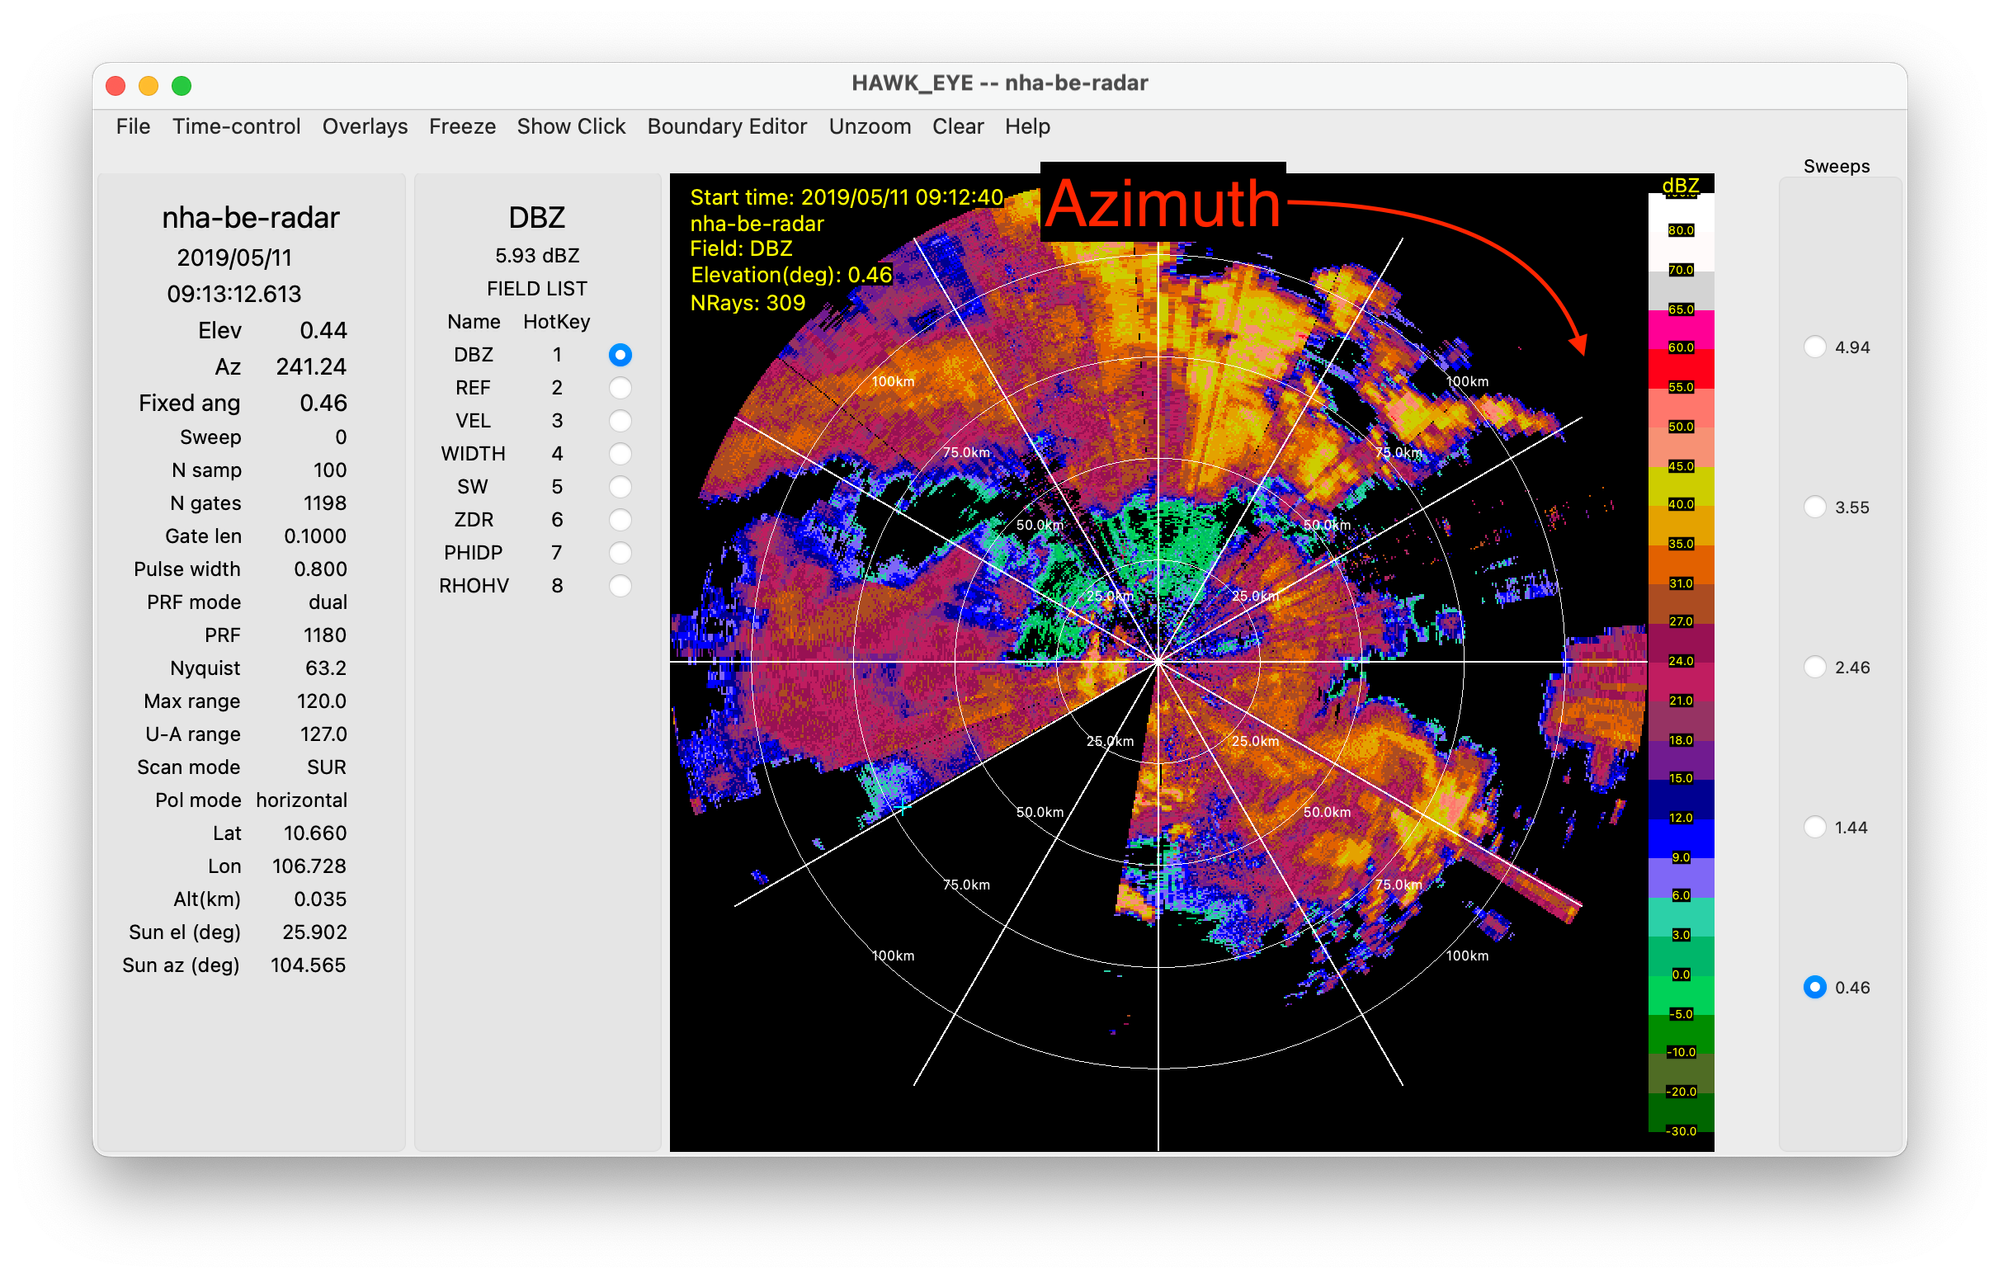
\includegraphics[width=0.8\linewidth]{Images/3.5-hawk-eye.png}
    \caption{Hawk Eye, Lidar and Radar visualization tool of LROSE}
    \label{fig:hawk-eye}
\end{figure}

The project actively encourages participation from a large scientific community, promoting the exchange of ideas, algorithms, and improvements for the software. Regular updates and contributions from users contribute to the continuous development and refinement of LROSE.

\subsection{FastAPI}
FastAPI is a high-performance web development framework based on Python, distinguished by its unique and advanced technical features designed to address challenges in building high-performance and flexible APIs.

It is one of the rare frameworks that fully leverages type hints and async/await. Type hints help clearly define the data types of variables and functions, making the source code more explicit and understandable. Additionally, support for async/await enables handling multiple requests concurrently without slowing down the processing, especially crucial for applications requiring high responsiveness and scalability.

With robust support for type hints, FastAPI automatically generates API documentation based on Python's data types. This not only helps reduce errors in the source code but also generates automatic API documentation, streamlining the development process and interaction with the API. FastAPI also supports industry standards such as OpenAPI and Swagger, providing a flexible way to manage resources, authentication, and user accounts.

Beyond its technical prowess, FastAPI excels in concurrent handling and performance. The special support from asyncio allows FastAPI to process multiple requests simultaneously without impeding processing speed. This capability ensures smooth and fast-running applications while facilitating scalability, a crucial factor for large research projects with evolving requirements over time.

FastAPI not only simplifies the development process but is also designed with the goal of optimizing the development experience. It lays the foundation for easily building production-ready APIs thanks to its integrated best practices. With this combination, FastAPI is not just a powerful tool but also an efficient and flexible solution for projects that demand reliability and scalability in the future.